\chapter{Modify a Rocket Chip RISC-V}\label{chap:mod_risc-v}
When it comes to implementing a feature in hardware one
needs to choose a modifiable processor implementation.
In this thesis, the Rocket Chip project was chosen, as it
seems to be most popular RISC-V implementation as of the time of this thesis.
The University of Berkeley and SiFive maintain the Rocket
Chip SoC generator and the Rocket core. Thus the project has
great support from the founders
and from a growing company that already has taped out
the Rocket cores twice.
The programming language of the Rocket Chip project
Chisel also seems to be a good fit for the job of
modifying the processor. The wide configurability of
the SoC generator also allows us to work on a
minimal base processor without additional distractions.
The rocket-chip GitHub repository can be found here
\footnote{\url{https://github.com/freechipsproject/rocket-chip}}.

\section{SiFive web configuration}
For a company that wants to evaluate RISC-V processors
the entry point of the programmed Chisel configuration might
be too high.
SiFive is creating a solution to this problem.
They are currently developing a product called
SiFive Core Designer which makes configuring a
processor easy.
In the current state of the website, we can choose
from three series of processors with different
submodels.
(ordered from low to high performance)
\begin{itemize}
    \item E20, E21, E24, E2 custom
    \item E31, E34, E3 custom
    \item S51, S54, S5 custom
\end{itemize}
\cite{sifive_core_designer} \newline
These models predefine the size of the design and approximate
which ARM chip is comparable to it.
The website is still in the preview phase, and thus not all
SiFive processors are available. Especially the higher
performance models will be available in the future.
When we selected a processor type, the following site
presents us with a UI in which we can choose what
capabilities the processor should have.
A screenshot of the site can be seen in figure
\ref{fig:sifive_core_designer}.
\begin{figure}
    \centering
    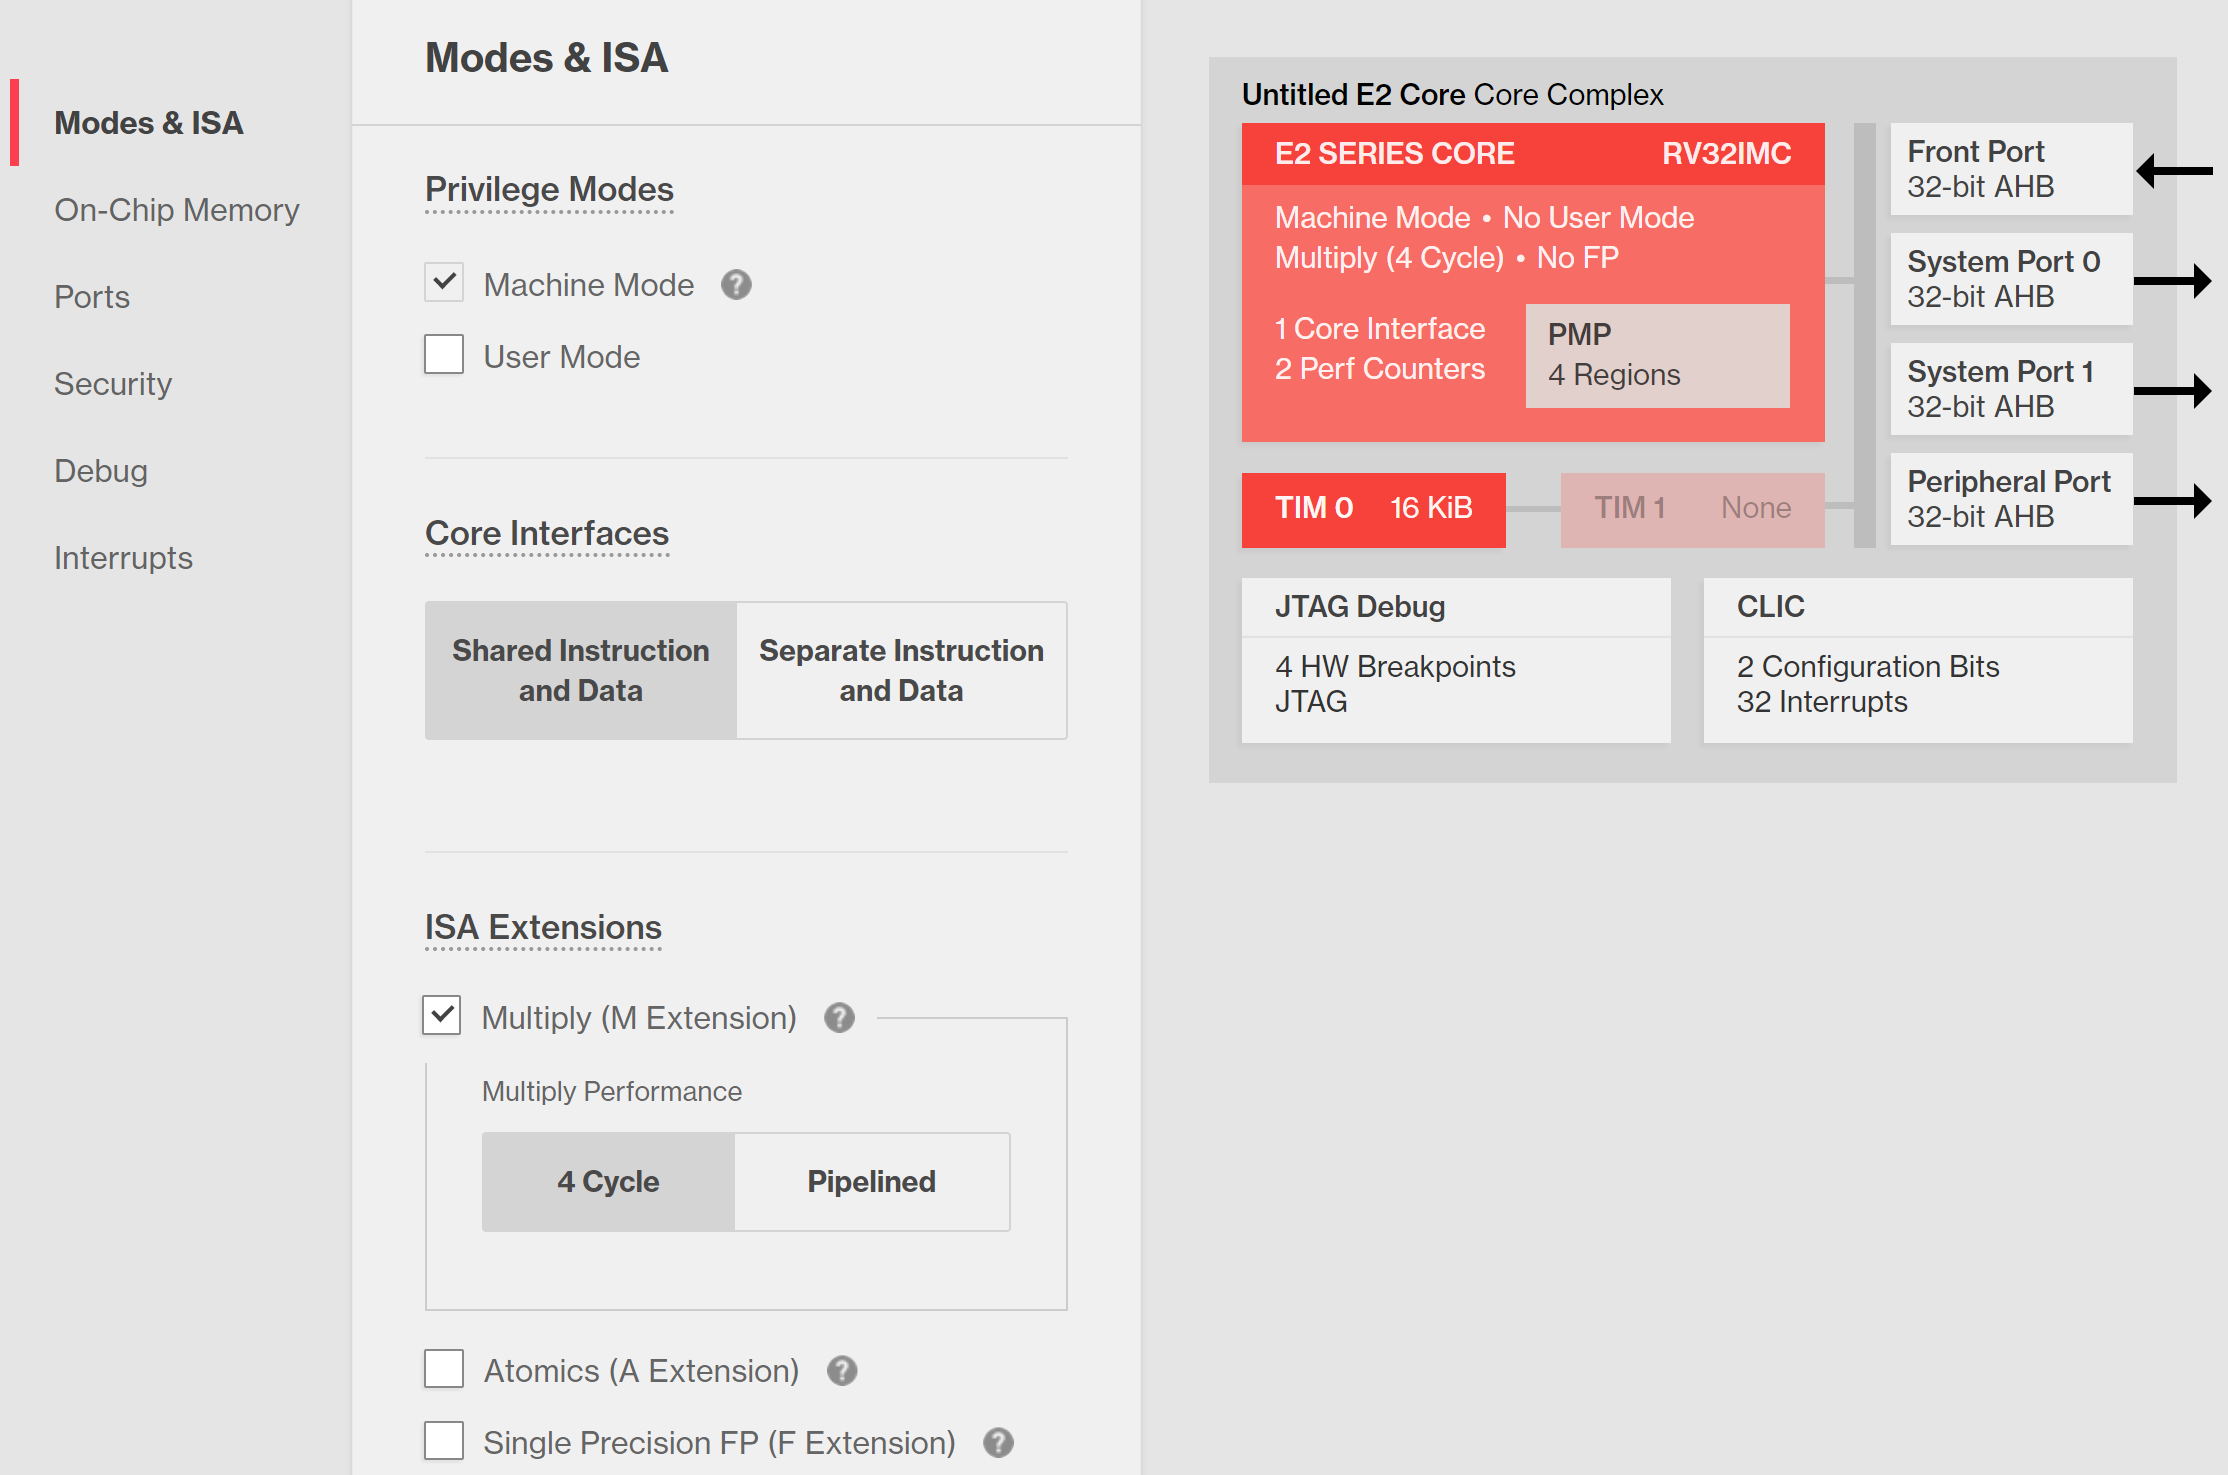
\includegraphics[width=0.9\textwidth]{figures/sifive_core_designer}
    \caption{The SiFive Core Designer \cite[Model: E20, connections added]{sifive_core_designer}}
    \label{fig:sifive_core_designer}
\end{figure}
We are presented with six menu items which allow us
to for example define what I/O ports the design should have.
Changes in the program display live in the interactive
presentation

\section{Standard Configuration}
If one wants to dive further in customizing RISC-V designs,
the standard configuration written in Chisel is the easiest way to 
modify the generated SoC. The configuration file which is located
at \textit{rocket-chip/src/main/scala/system/Configs.scala} provides
the developer with configurations that already have been proven to work.
To generate a standard single Rocket core
the configuration
\begin{lstlisting}[language=scala, frame=single]
    class DefaultConfig extends Config(new WithNBigCores(1) ++ new BaseConfig)
\end{lstlisting}
can be used. A quadcore processor is generated if the developer changes the
1 to a 4.
To get a better understanding of the configuration process
let us inspect the class WithNBigCores(n: Int).
\begin{lstlisting}[language=scala, frame=single]
    class WithNBigCores(n: Int) extends Config((site, here, up) => {
        case RocketTilesKey => {
            val big = RocketTileParams(
              core   = RocketCoreParams(mulDiv = Some(MulDivParams(
                mulUnroll = 8,
                mulEarlyOut = true,
                divEarlyOut = true))),
              dcache = Some(DCacheParams(
                rowBits = site(SystemBusKey).beatBits,
                nMSHRs = 0,
                blockBytes = site(CacheBlockBytes))),
              icache = Some(ICacheParams(
                rowBits = site(SystemBusKey).beatBits,
                blockBytes = site(CacheBlockBytes))))
        List.tabulate(n)(i => big.copy(hartId = i))
        }
    })
\end{lstlisting}
In the piece of code above a standard configuration
is described.
We define a freely named variable big, which
resembles one tile in our SoC design.
Following we define, that the Rocket core should
have a multiply and divide module (mulDiv).
We continue with the size of the data cache (dcache)
and instruction cache (icache).
Additionally, we define that the data cache should
be blocking (nMSHRs = 0).
The last line in the example code duplicates
the previously defined tile n times and
assigns each new tile an ascending hardware thread
number (hartId).
The Rocket core above will be an all-purpose core
which can, for example, execute Linux.
In comparison, we can also configure a Rocket core
for the use in a microcontroller.
\begin{lstlisting}[language=scala, frame=single]
    class DefaultSmallConfig extends Config(
        new WithNSmallCores(1) ++
        new BaseConfig
    )

    class WithNSmallCores(n: Int) extends Config((site, here, up) => {
        case RocketTilesKey => {
        val small = RocketTileParams(
            core = RocketCoreParams(useVM = false, fpu = None),
            btb = None,
            dcache = Some(DCacheParams(
                rowBits = site(SystemBusKey).beatBits,
                nSets = 64,
                nWays = 1,
                nTLBEntries = 4,
                nMSHRs = 0,
                blockBytes = site(CacheBlockBytes))),
            icache = Some(ICacheParams(
                rowBits = site(SystemBusKey).beatBits,
                nSets = 64,
                nWays = 1,
                nTLBEntries = 4,
                blockBytes = site(CacheBlockBytes))))
        List.tabulate(n)(i => small.copy(hartId = i))
        }
    })
\end{lstlisting}
Again we define a tile but this time it should be smaller.
To achieve this, we disable the creation of
the FPU and set the parameter useVM to false.
The name useVM might be a bit misleading here.
It does not reference the hypervisor capability of the
Rocket core but controls the creation of an MMU.
Thus this processor will
not have the capability of using a virtual address space.
As in our previous design, we now define the sizes of the
data and instruction cache, but override the standard value
\textit{nWays}=4 with 1 to get a 1-way associated cache, which results
in slimmer data interconnects and thus a simpler CPU.
Again, as the last step, the design is duplicated and
the according hartId is assigned.

\section{Rocket Custom Coprocessor (RoCC)}
If the above methods do not fulfill the requirements
of the use case, more custom accelerators can be added to
the design. A comparably easy way to do this is to use
the Rocket Custom Coprocessor (RoCC) interface.
The RoCC interface defines how the accelerator is
connected and how it can be called.
\begin{figure}
    \centering
    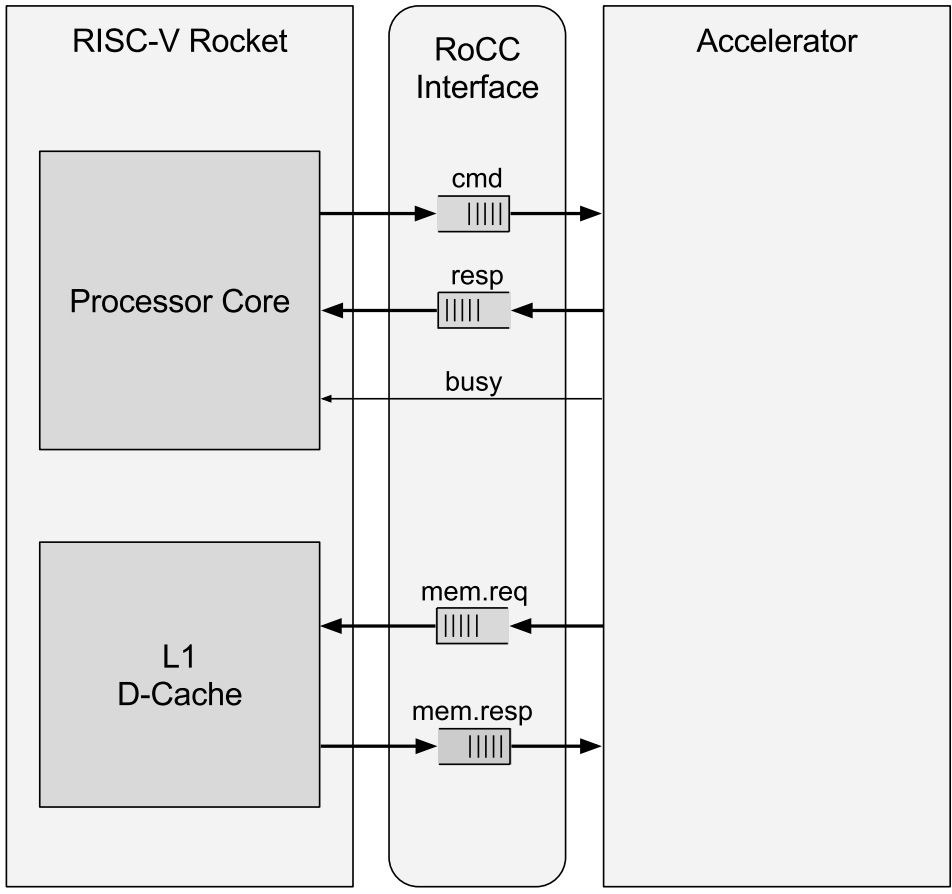
\includegraphics[width=0.6\textwidth]{figures/rocket_chip_rocc_simple}
    \caption{Simplified view on a processor with RoCC accelerator \cite[p.~6]{rocket_chip_rocc_presentation}}
    \label{fig:rocket_chip_rocc_simple}
\end{figure}
In figure \ref{fig:rocket_chip_rocc_simple} a simplified Rocket
core with a connected RoCC accelerator can be seen.
Although the accelerator in the figure is only connected
to the L1 data cache, a connection to the L2 cache or
another component block is possible.
Again as in the previous section, everything is designed
and configured with Chisel.

\section{Standard extension}
If additional changes to the execution have to
be made, we need to go deeper into
the code of Rocket Chip.
All changes that need to be made to the existing
code should be made optional.
If we, for example, need additional registers
for our task, we would need to place
checks for our extension in the code.
If the extension is deactivated, the generated
design does not contain any hints to the
existence of the extension.

\section{Non-standard extensions}
If a change to the code cannot be made optional,
the last resort is to generate a non-standard
extension patch for the Rocket Chip project.
The design of the generated chip is defined in
the code after all, and as the code is licensed
freely, everthing can be done with it.
The downside to this approach is, that future
version and other standards of the ISA might no
longer be compatible to the non-standard changes.